\documentclass[9pt]{extarticle}
\usepackage[margin=0.7cm]{geometry}
\usepackage[UKenglish]{babel}
\usepackage{parallel,enumitem}
\usepackage{multicol}
\setlength{\columnsep}{0.7cm}
\setlength{\columnseprule}{0.5pt}
\usepackage{amssymb}
\usepackage{amsmath}
\usepackage{bm}
\usepackage{graphicx}
\graphicspath{{./pics/}}
\usepackage{physics}

%% vectors and matrices
\renewcommand{\v}[1]{{\bm #1}}
\renewcommand{\dv}[1]{\dot{\bm{#1}}}
\newcommand{\ddv}[1]{\ddot{\bm{#1}}}
\newcommand{\hv}[1]{\hat{\bm{#1}}}
\newcommand{\m}[1]{[ #1 ]}
\renewcommand{\t}[1]{\widetilde{\bm{#1}}}
\newcommand{\bfit}[1]{\textbf{\textit{#1}}}

%% differential and integral operators
\renewcommand{\d}{\text{d}}
\renewcommand{\dd}[2]{\frac{\d #1}{\d #2}}
\newcommand{\ddd}[2]{\frac{\d^2 #1}{\d #2^2}}
\newcommand{\ddt}[1]{\frac{\d #1}{\d t}}
\newcommand{\dddt}[1]{\frac{\d^2 #1}{\d t^2}}
\newcommand{\pd}[2]{\frac{\partial #1}{\partial #2}}
\newcommand{\pdd}[2]{\frac{\partial^2 #1}{\partial #2^2}}
\renewcommand{\grad}{\boldsymbol \nabla} 
\renewcommand{\div}{\boldsymbol \nabla \cdot}
\renewcommand{\curl}{\boldsymbol \nabla \times}
\newcommand{\lap}{\nabla^2}

%% constants
\newcommand{\eo}{\epsilon_0}
\newcommand{\muo}{\mu_0}

%% statistics
\newcommand{\E}{\text{E}}
\newcommand{\Var}{\text{Var}}
\newcommand{\SD}{\text{SD}}
\newcommand{\SE}{\text{SE}}
\newcommand{\Cov}{\text{Cov}}
\newcommand{\Cor}{\text{Cor}}
\renewcommand{\P}{\text{P}}
\newcommand{\Bias}{\text{Bias}}

\begin{document}

\setlength{\parindent}{0pt}

{\huge \bf problem set} 

\noindent \hrulefill

\begin{multicols*}{2}

{\LARGE \bf I --- Spherical Resistor} \\

Consider a resistor with conductivity $\sigma$ filling the space between two concentric spherical shells with radii $a$ and $b$. \\ 

\begin{center}
	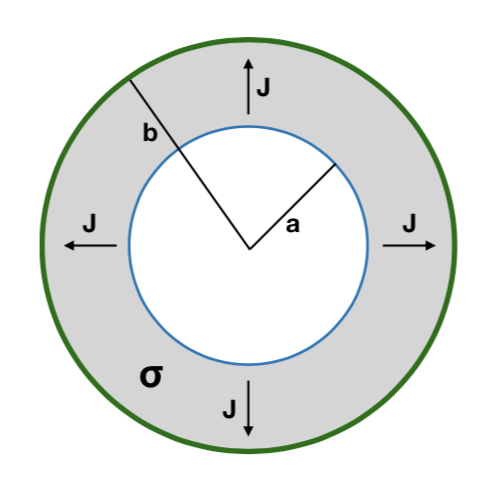
\includegraphics[scale=0.5]{ps7-pic1.png}
\end{center}

{\Large \bf a.} If the shells are maintained at potential difference $V$, what current flows from one shell to the other? \\ 

{\bfit{Solution}} \\ 

If $q$ is the charge on the inner shell, then the electric field in the space between the shells is:

$$\v E = \frac{1}{4\pi\eo} \frac{q}{r^2} \hv r$$ \ 

Using Ohm's law, $\v J = \sigma \v E$, and the fact that current is related to current density by $I = \int \v J \cdot \d \v a$, the current flowing between the shells is:

$$I = \int \v J \cdot \d a = \sigma \int \v E \cdot \d a = \sigma \frac q\eo$$ \ 

Note the potential difference between the shells is:

$$\Delta V = V_a - V_b = -\int_b^a \v E \cdot \d \v r = -\frac{q}{4\pi\eo} \int_b^a \frac{1}{r^2} \d r = \frac{q}{4\pi\eo} \bigg( \frac 1a - \frac 1b \bigg)$$ \ 

Thus the charge $q$ can be expressed in terms of potential difference as:

$$q = \frac{4\pi\eo \Delta V}{\frac 1a - \frac 1b}$$ \ 

Substituting this into the equation above for current:

$$I = \frac{\sigma 4\pi \Delta V}{\frac 1a  - \frac 1b}$$ \ 

where $\Delta V = V_a - V_b$. \\  



\dotfill 

\hfill 

{\Large \bf b.} What is the resitance between the shells? \\ 

{\bfit{Solution}} \\ 

From Ohm's law:

$$R = \frac{\Delta V}{I} = \frac{1}{4\pi\sigma} \bigg( \frac 1a - \frac 1b \bigg)$$ \ 



\dotfill 

\hfill 

{\Large \bf c.} Suppose we change the problem such that the conductivity is no longer uniform. Let's suppose $\sigma(r) = \frac{k}{r^2}$. Find the new resistance $R$ between the shells. {\it Hint:} Since $\sigma$ is not uniform, $\div E \neq \frac{\div J}{\sigma}$ and $\rho_e \neq 0$ in the resistive medium. This alters the behaviour of $\v E$ in the medium. However, you can still use the fact that $I$ is the same across any spherical surface. \\  

{\bfit{Solution}} \\ 

Resistance is given by Ohm's law as $R = \frac VI$. To find resistance we must first find $V$ and $I$. \\ 

Current is related to current density by $I  = \int \v J \cdot \d \v a$, and by Ohm's law $\v J = \sigma \v E$, thus:

$$I = \int \v J \cdot \d \v a = \int \sigma \v E \cdot \d \v a = \int \frac{k}{r^2} \frac{q}{4\pi \eo r^2} r^2\sin\theta \d\theta \d\phi$$ 

$$= \frac{kq}{4\pi\eo r^2} \int_0^\pi \sin\theta \d\theta \int_0^{2\pi} \d\phi = \frac{kq}{\eo r^2}$$ \ 

And, since $I  = \frac{kq}{\eo r^2}$, this means $q = \frac{I\eo r^2}{k}$, and the electric field can thus be expressed:

$$\v E = \frac{1}{4\pi} \frac Ik$$ \ 

The potential is:

$$V = -\int_b^a \v E \cdot \d \v r = -\int_b^a  \frac{1}{4\pi} \frac Ik \d r = \frac{I}{4\pi k} (b-a)$$ \ 

And, using Ohm's law, the resistance between the shells is thus:

$$R = \frac VI = \frac{b-a}{4\pi k}$$ \ 






\hrulefill 

\hfill 

{\LARGE \bf II --- RC Circuit} \\ 

{\it Griffiths 7.2} \\ 

A capacitor $C$ has been charged up to potential $V_0$; at time $t=0$, it is connected to a resistor $R$, and begins to discharge. \\ 

\begin{center}
        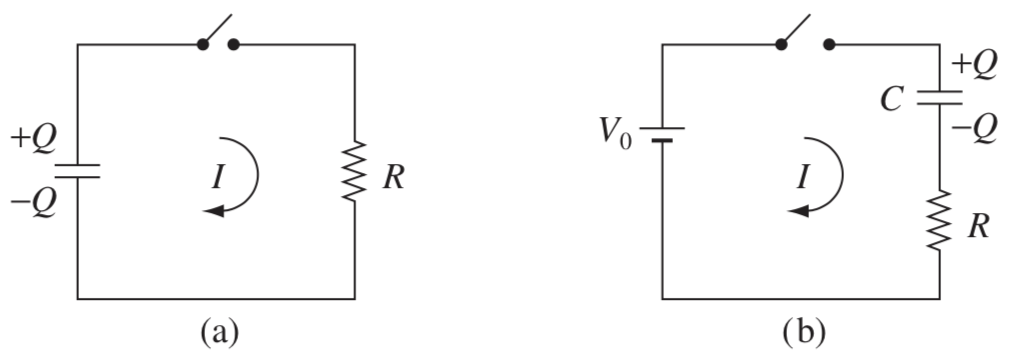
\includegraphics[scale=0.5]{ps7-pic2.png}
\end{center}

{\Large \bf a.} Determine the charge on the capacitor as a function of time, $Q(t)$. What is the current through the resistor, $I(t)$? \\ 

{\bfit{Solution}} \\ 

The potential of a capacitor is $V = \frac QC$, and Ohm's law gives $V=IR$. This means $I = \frac{Q}{RC}$, and thus the charge as a function of time is:

$$Q(t) = \int -I \d t=  \int -\frac{Q}{RC} \d t = Q_0 e^{-t/RC}$$ \ 

The initial charge at time $t=0$ is $Q_0 = CV_0$, thus:

$$Q(t) = CV_0 e^{-t/RC}$$ \ 

From Ohm's law, the current through the resistor is $I = \frac VR = \frac{Q}{RC}$. As a function of time this is:

$$I(t) = \frac{Q(t)}{RC} = \frac{V_0}{R} e^{-t/RC}$$ \ 



\dotfill 

\hfill 

{\Large \bf b.} What was the original energy stored in the capacitor (eq. 2.55)? By integrating eq. 7.7, confirm that the heat delivered to the resistor is equal to the energy lost by the capacitor. \\ 

{\bfit{Solution}} \\ 

From eq. 2.55, the original energy stored in the capacitor at time $t=0$ was:

$$W = \frac 12 CV_0^2$$ \ 

From eq. 7.7, power is given by $P = VI = I^2 R$. The heat delivered to the resistor is:

$$\int_0^\infty P \d t = \int_0^\infty I^2 R \d t = \frac{V_0^2}{R} \int_0^\infty e^{-2t/RC} \d t$$

$$= \frac{V_0^2}{R} \bigg( -\frac 12 RC e^{-2t/RC} \bigg) \bigg|_0^\infty = \frac 12 CV_0^2$$ \ 



\dotfill 

\hfill 

{\Large \bf c.} Next, imagine {\it charging up} the capacitor, by connecting it (and the resistor) to a battery of voltage $V_0$, at time $t=0$ (fig b). Again, determine $Q(t)$ and $I(t)$. \\  

{\bfit{Solution}} \\ 

For a charging capacitor, the initial charge on the capacitor is zero, and the final charge is $CV_0$. From the answer in part (a), we can logically deduce that the charge as a function of time must be:

$$Q(t) = CV_0(1 - e^{-t/RC})$$ \ 

It also follows that the current as a function of time is simply:

$$I(t) = \frac{V_0}{R} e^{-t/RC}$$ \ 



\dotfill 

\hfill 

{\Large \bf d.} Find the total energy output of the battery, $\int V_0 I \d t$. Determine the heat delivered to the resistor. What is the final energy stored in the capacitor? What fraction of the work done by the battery shows up as energy in the capacitor? Note that the answer is independent of $R$. \\ 

{\bfit{Solution}} \\ 

The total energy output of the battery is:

$$\int_0^\infty V_0 I \d t = \frac{V_0^2}{R} \int_0^\infty e^{-t/RC} \d t = \frac{V_0^2}{R} \big( -RC e^{-t/RC} \big) \bigg|_0^\infty = CV_0^2$$ \ 

The current as a function of time is:

$$I(t) = \frac{V_0}{R} e^{-t/RC}$$ \ 

It follows that the heat delivered to the resistor is $\frac 12 CV_0^2$ and the final energy stored by the capacitor is also $\frac 12 CV_0^2$. In other words, {\it half} the work done by the battery shows up as energy in the capacitor. \\ 








\hrulefill 

\hfill 

{\LARGE \bf III --- Motional EMF} \\ 

{\it Griffiths 7.8} \\ 

A square loop of wire (side $a$) lies on a table, a distance $s$ from a very long straight wire, which carries a current $I$. \\  

\begin{center}
        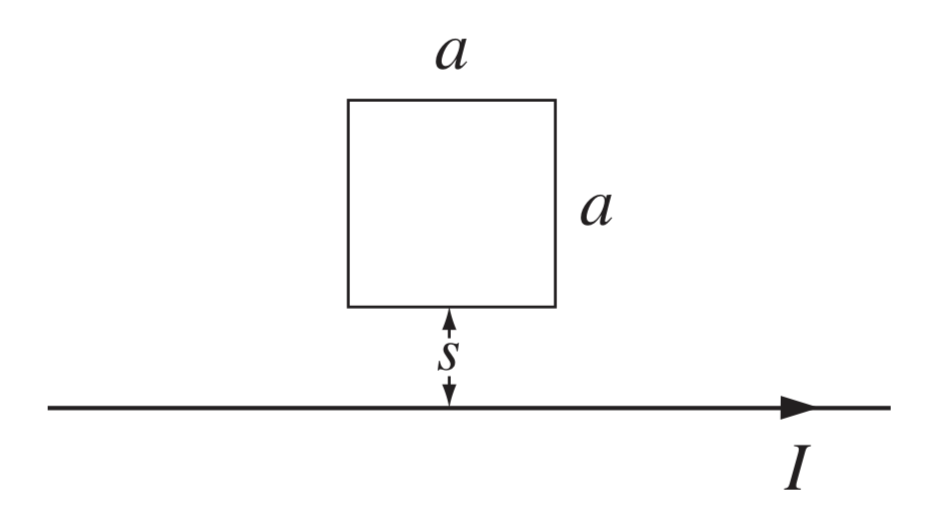
\includegraphics[scale=0.3]{ps7-pic3.png}
\end{center}

{\Large \bf a.} Find the flux of $\v B$ through the loop. \\ 

{\bfit{Solution}} \\ 

The field of the wire, given by Ampère's law, is:

$$\v B = \frac{\muo I}{2\pi s} \hv \phi$$ \ 

The flux of $\v B$ through the loop is thus:

$$\Phi_B = \int \v B \cdot \d \v a = \frac{\muo I}{2\pi} \int_s^{s+a} \frac as \d s$$

$$= \frac{\muo Ia}{2\pi} \ln \bigg( \frac{s+a}{s} \bigg)$$ \ 



\dotfill 

\hfill 

{\Large \bf b.} If someone now pulls the loop directly away from the wire, at speed $v$, what emf is generated? In what direction (clockwise or anticlockwise) does the current flow? \\ 

{\bfit{Solution}} \\ 

Faraday's law gives the emf $\varepsilon = -\ddt \Phi$. Using the answer from part (a):

$$\varepsilon = \ddt{} \Bigg[ -\frac{\muo Ia}{2\pi} \ln \bigg( \frac{s+a}{s} \bigg) \Bigg] = -\frac{\muo Ia}{2\pi} \ddt{} \bigg( \ln (s+a) - \ln(s) \bigg)$$ \ 

Using the fact that $\ddt s = v$, the expression above becomes:

$$\varepsilon = -\frac{\muo  I a}{2\pi} \bigg( \frac{1}{s+a} \ddt s - \frac 1s \ddt s \bigg) = \frac{\muo I a^2 v}{2\pi s(s+a)}$$ \ 

Since the field points out of the page, the force on the loop acts {\it rightwards}, and Lenz's law gives the direction of the induced current as {\it anticlockwise}. \\ 



\dotfill 

\hfill 

{\Large \bf c.} What if the loop is pulled to the {\it right} at speed $v$? \\ 

{\bfit{Solution}} \\ 

If the loop is being pulled to the right, the flux through it is constant, and so the induced emf is zero. 

$$\varepsilon = 0$$ \ 



\dotfill 

\hfill 

{\Large \bf d.} Place the loop under  the wire with the centre of the loop a distance $d$ from the wire. The wire is then released from rest, only to fall under the influence of gravity. Assume the loop has a resistance $R$. Find the current flowing in the wire as a function of time. Include the direction. \\ 

{\bfit{Solution}} \\ 

The field at distance $d$ from the wire is given by Ampère's law as:

$$\v B = \frac{\muo I}{2\pi r}$$ \ 

The total flux through the loop, when at a distance $d$ from the wire, is:

$$\Phi = \frac{\muo I a}{2\pi} \int_{d - a/s}^{d+a/2} \frac 1r \d r = \frac{\muo Ia}{2\pi} \ln \bigg( \frac{2d+a}{2d-a} \bigg)$$ \  

Faraday's law gives the induced emf as:

$$\varepsilon = -\ddt{\Phi_B} = -\frac{\muo a}{2\pi} \ln \bigg( \frac{2d+a}{2d-a} \bigg) \ddt I$$ \ 

And, thus, the current in the loop is:

$$I(t) = -\frac{\muo a}{2\pi R} \ln \bigg( \frac{2d+a}{2d-a} \bigg) \ddt I$$ \ 

where $\ddt I$ is the rate of change of current in the {\it straight} wire. \\ 






\hrulefill 

\hfill 

{\LARGE \bf IV --- Faraday Induced EMF} \\ 

\begin{center}
        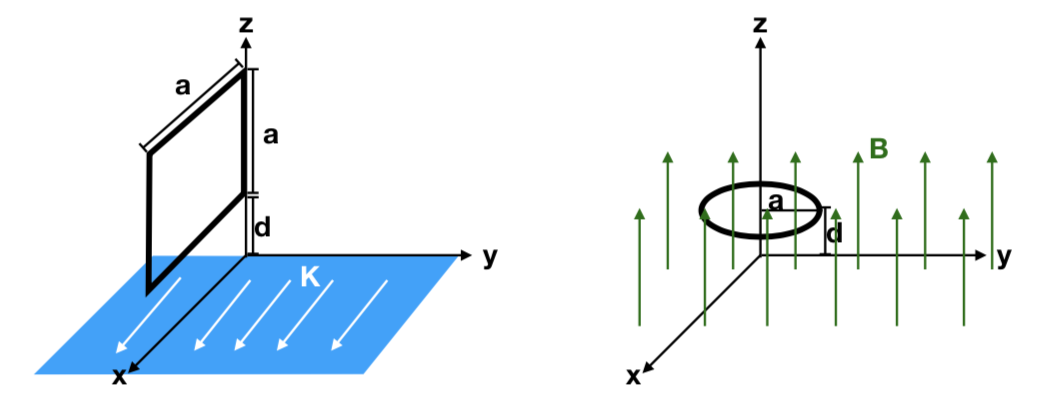
\includegraphics[scale=0.5]{ps7-pic4.png}
\end{center}

{\Large \bf a.} A time-dependent areal current density  $K = \alpha\sin(\beta t)$ flows in the  $x$-direction on a sheet in the $xy$ plane. A square loop of wire with resistance $R$ and side length $a$ is in the $xz$ plane, with its bottom side a distance $d$ above the current sheet. Find the time-dependent current (magnitude and direction) in the loop. \\ 

{\bfit{Solution}} \\ 

For $z>0$, the field due to the current sheet is:

$$\v B = \frac{\muo K}{2} (-\hv y)$$ \ 

The flux through the loop is thus:

$$\Phi_B = \int \v B \cdot \d \v a = \frac{\muo Ka^2}{2}$$ \ 

Faraday's law gives the induced emf as:

$$\varepsilon = -\ddt{\Phi_B} = -\frac{\muo a^2}{2} \alpha \ddt{} \sin \beta t = -\frac{\muo a^2}{2} \alpha\beta\cos \beta t$$ \ 

Ohm's law gives the current as $I = \frac VR$, in this case:

$$I(t) = \frac{\muo a^2}{2R} \alpha \beta \cos \beta t$$ \ 

Lenz's law gives that the direction of the induced current as that which opposes the change in flux (which in this case oscillates). \\ 



\dotfill 

\hfill 

{\Large \bf b.} A circular loop of radius $a$, a distance $d$ above the origin and the $xy$ plane, is in a magnetic field $\v B = ks^3 z \sin \frac \phi 3 \cos\omega t \hv z$ (cylindrical coordinates), where $k$ is  a constant. Find the  emf in  the loop. \\ 

{\bfit{Solution}} \\ 

The field at $z=d$ is:

$$\v B = ks^3 d \sin \frac \phi 3 \cos \omega t \hv z$$ \ 

The flux through the loop is:

$$\Phi_B = \int \v B \cdot \d \v a = kd \cos \omega t \int s^3 \sin \frac \phi 3 s \d s \d\phi$$

$$= kd\cos\omega t \bigg[ \frac{s^5}{5} \bigg]^a_0 \bigg[-3\cos\frac \phi 3 \bigg]_0^{2\pi} = -\frac{9}{10} kda^5 \cos\omega t$$ \ 

Faraday's law gives the induced emf in the loop as:

$$\varepsilon = -\ddt{\Phi_B} = \frac{9}{10} kda^5 \omega \sin\omega t$$ \ 


 
\dotfill 

\hfill 

{\Large \bf c.} A circular loop of radius $a$ and resistance $R$ in the $xy$ plane is in  a uniform, constant magnetic field pointing in the $z$-direction. Suddenly the magnetic field turns off. How much charge passes through the loop during the current flow? \\ 

{\bfit{Solution}} \\ 

Turning off the magnetic field causes a change in flux:

$$\Delta \Phi_B = \Phi_B \; \text{(final)}  - \Phi_B \; \text{(initial)}  = -B\pi a^2$$ \ 

Faraday's law gives the induced emf as:

$$-\ddt{\Phi_B} = \ddt{} B\pi a^2$$ \ 

The charge that passes through the loop during the current flow is:

$$\d q = I\d t = \frac VR \d t = \frac{\ddt{} B\pi a^2}{R} \d t = \frac{B\pi a^2}{R}$$ \ 







\hrulefill 

\hfill 

{\LARGE \bf V --- Induced Electric Fields} \\ 

{\it Griffiths 7.15} \\  

A long solenoid with radius $a$ and $n$ turns per unit length carries a time-dependent current $I(t)$ in the $\hv \phi$ direction. Find the electric field (magnitude and direction) at a distance $s$ from the axis (both inside and outside the solenoid), in the quasistatic approximation. \\ 

{\bfit{Solution}} \\ 

In the quasistatic approximation, the field in the  solenoid is:

$$
\v B = 
\begin{cases}
	\muo n I \hv z & s < a \\ 
	0 & s > a 
\end{cases}
$$ \ 

Inside the loop, Ampère's law gives: 

$$\Phi_B = \int \v B \cdot \d \v a = B\pi s^2  = \muo n I \pi s^2$$ \ 

Faraday's law gives:

$$\oint \v E \cdot \d \v l = -\ddt{\Phi_B}$$ \ 

where, in this case 

$$\oint \v E \cdot \d \v l = E2\pi s$$

$$-\ddt{\Phi_B} = -\ddt{} \big( \muo nI\pi s^2 \big) = -\muo n\pi s^2 \ddt I$$ \ 

Thus:

$$E2\pi s = -\muo n\pi s^2 \ddt I$$ \ 

and the electric field {\it inside} the solenoid is:

$$ \v E = -\frac 12 \muo ns \ddt I \hv \phi$$ \\ 

Outside the loop, Ampère's law gives:

$$\Phi_B = \int \v B \cdot \d \v a = B\pi a^2 = \muo nI \pi a^2$$ \ 

And, in this case:

$$\oint \v E \cdot \d \v l = E2\pi s$$

$$-\ddt{\Phi_B} = -\ddt{} \muo nI \pi a^2 = -\muo n\pi a^2 \ddt I$$ \ 

Using Faraday's law:

$$E2\pi s = -\muo n\pi a^2 \ddt I$$ \ 

and the electric field {\it outside} the solenoid is:

$$\v E = -\frac{1}{2s} \muo na^2 \ddt I \v \phi$$ \\ 

Thus the electric field inside and outside the solenoid is:

$$
\v E = 
\begin{cases}
	 -\frac 12 \muo ns \ddt I \hv \phi & s < a \\
	\\  
	 -\frac{1}{2s} \muo na^2 \ddt I \hv \phi & s > a
\end{cases}
$$ \ 









\hrulefill 

\hfill 

{\LARGE \bf VI --- Variable Toroid} \\ 

{\it Griffiths 7.19} \\ 

A toroidal coil has a rectangular cross section, with inner radius $a$, outer radius $a+w$, and height $h$. It carries a total of $N$ tightly wound turns, and the current is increasing at a constant rate,  i.e. $\ddt I = k$. If $w$ and $h$ are both much less than $a$, find the electric field at a point $z$ above the centre of the toroid. {\it Hint:} exploit the analogy between Faraday fields and magnetostatic fields, and refer to ex. 5.6. \\ 

{\bfit{Solution}} \\ 

The magnetic field inside and outside a toroid is given by Ampère's law as:

$$\v B = 
\begin{cases}
	\frac{\muo NI}{2\pi s} \hv \phi & \text{inside} \\ 
	\\ 
	0 & \text{outside} 
\end{cases}
$$ \ 

The flux around the toroid is:

$$\Phi_B = \int \v B \cdot \d \v a = \frac{\muo NI}{2\pi} \int_a^{a+w} \frac hs \d s =  \frac{\muo NI h}{2\pi} \ln \bigg( 1 + \frac wa \bigg)$$

$$\approx \frac{\muo NIhw}{2\pi a}$$ \ 

Given the shape of the toroid, the expression for the electric field is equivalent to that for the magnetic field of a circular current:

$$\v E = \frac 12 \muo  I \frac{a^2}{(a^2+z^2)^{3/2}} \hv z$$ \ 

Using Faraday's law, we can see that the current $I$ can be expressed:

$$I  = -\frac{1}{\muo} \ddt{\Phi_B} = -\frac{Nhwk}{2\pi a}$$ \ 

Substituting this into the expression for electric field above gives:

$$\v E = -\frac{\muo}{4\pi} \frac{Nhwka}{(a^2+z^2)^{3/2}} \hv z$$ \ 

\end{multicols*}

\end{document}
